\documentclass[12pt,a4paper]{article} 

\usepackage[spanish]{babel} 
\usepackage[utf8]{inputenc}
\usepackage[numbers,sort&compress]{natbib} 
\usepackage{graphicx} 
\usepackage{amsfonts}
\usepackage[left=2cm,right=2cm,top=2cm,bottom=2cm]{geometry}
\usepackage{listings}
\usepackage[usenames,dvipsnames]{color}
\lstset{ 
  language={R},
  basicstyle=\scriptsize\ttfamily,
  numbers=left,
  numberstyle=\tiny\color{Blue},
  stepnumber=1,
  numbersep={4pt},
  backgroundcolor=\color{white},
  showstringspaces=false,
  showtabs=false,
  frame=single,
  rulecolor=\color{black},
  tabsize=2,
  captionpos=b,
  breaklines=true,
  breakatwhitespace=false,        
  keywordstyle=\color{RoyalBlue},
  commentstyle=\color{YellowGreen},
  stringstyle=\color{ForestGreen}
}

\title{Matemáticas Computacionales \\ Práctica 2: Estudio de una base de datos} 
\author{Brenda Esthela Martinez Martinez  1874537}

\begin{document}
\maketitle
\section{Introducci\'{o}n}\label{sec:intro}

El proposito de esta práctica es conocer algunas de las bases de datos que se encuentran en R y de una de estas poder crear un reporte en el que nos grafique los datos que contiene, asi como tambien investigas ejemplos para lo que son utilizadas estas bases de datos.

\section{Base de datos: Tasas de conversión de las monedas euro}\label{sec:DATABASE}
La base de datos \textbf{euro.cross} \cite{euro} nos brinda las tasas de conversiones entre monedas europeas. Es un matriz 11 por 11 que contiene los valores para convertir las monedas. 
\subsection{Contenido de la base de datos}
El conjunto de datos eurocontiene el valor de 1 euro en todas las monedas que participan en la unión monetaria europea.\cite{1streport}

		\textit{\textbf{Chelín austríaco ATS,
		Franco belga BEF,
		Marco alemán DEM,
		Peseta española ESP,
		Marco finlandés FIM,
		Franco francés FRF,
		Irish Punt IEP,
		Lira italiana ITL,
		Franco luxemburgués LUF,
		Florín holandés NLG y
		Escudo portugués PTE}
	}
		
Estas tasas de conversión fueron fijadas por la Unión Europea el 31 de diciembre de 1998. Para convertir los precios antiguos a precios en euros, divida por la tasa respectiva y redondee a 2 dígitos.

El conjunto de datos \textbf{euro.cross} contiene tasas de conversión entre las distintas monedas de euro, es decir, el resultado de  $ \frac{1}{euro}, euro $ . 

\subsection{Conversiones}
En el codigo del cuadro \ref{alg:C1} podemos observar ejemplos de como convertir algunas monedas con la base de datos \textbf{euro} y \textbf{euro.cross} y en la figura \ref{fig:R1} podemos observar el resultado que nos arroja el codigo. 
\begin{table}[htpb]
	\begin{lstlisting}
		## Convert 20 Euro to Belgian Franc
		20 * euro["BEF"]
		## Convert 20 Austrian Schilling to Euro
		20 / euro["ATS"]
		## Convert 20 Spanish Pesetas to Italian Lira
		20 * euro.cross["ESP", "ITL"]
	\end{lstlisting}
	\caption{Código en R para convertir algunas monedas}
	\label{alg:C1}
\end{table}
\begin{figure}
\centering
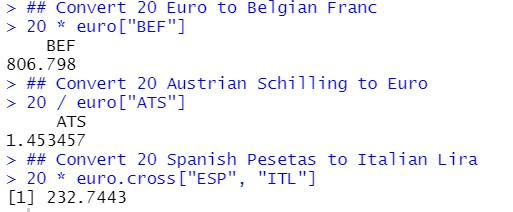
\includegraphics[scale=.8]{R1}
\caption{Resultados de la conversion}
\label{fig:R1}
\end{figure}
\newpage
\subsection{Grafico de la relacion del euro con las demas monedas europeas}
En la figura \ref{fig:G1} podemos observar la relacion que tiene el euro con otras de las monedas europeas que se encuntran en la base de datos y en la figura \ref{fig:T1} vemos el contenido completo de la base de datos.
\begin{figure}
\centering
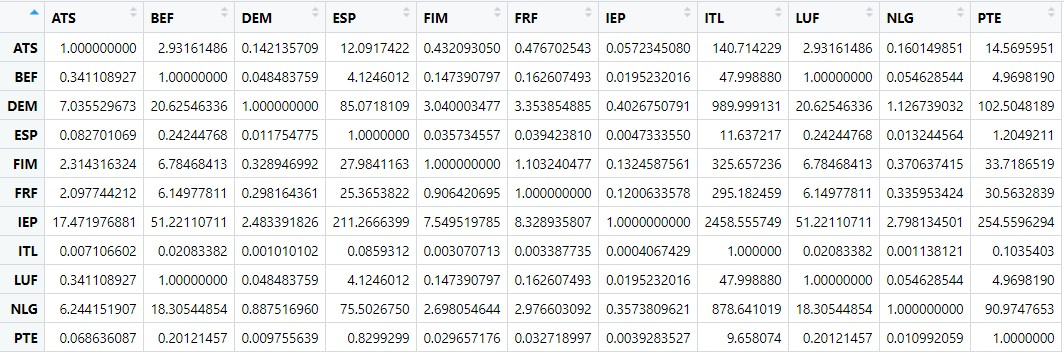
\includegraphics[scale=.6]{T1}
\caption{euro.cross}
\label{fig:T1}
\end{figure}
\begin{figure}
\centering
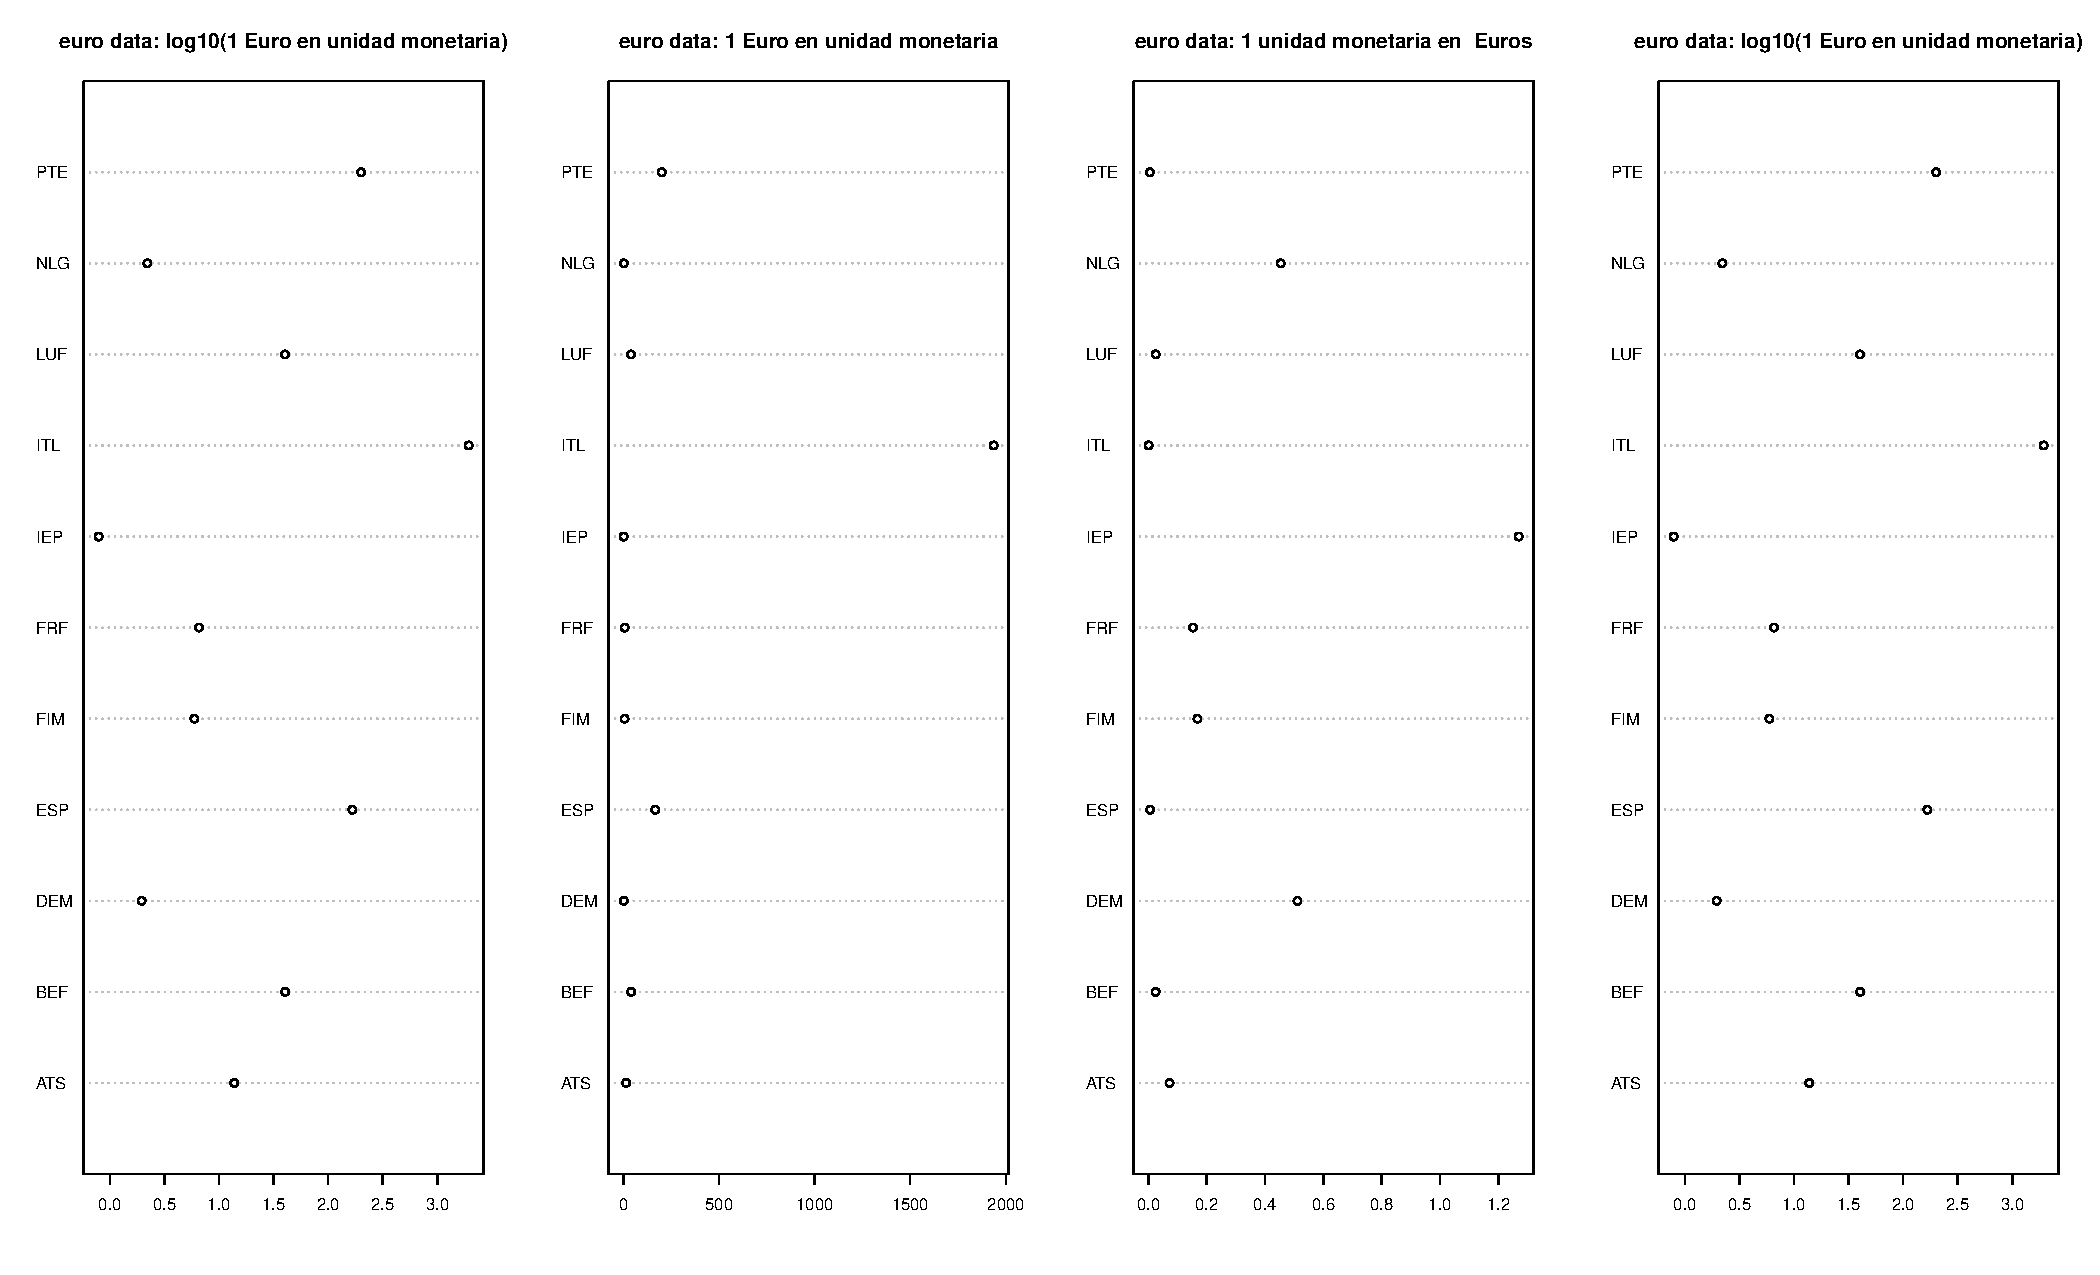
\includegraphics[scale=.5]{G1}
\caption{EURO VS OTRAS MONEDAS EUROPEAS}
\label{fig:G1}
\end{figure}
\newpage
\subsection{Summary/resumen}
El método de Summary muestra los valores mínimo y máximo en el conjunto de datos, el valor medio de cada columna de datos (el primer cuartil (Q1) significa que el $ 25 porciento $ de las observaciones están por debajo de esta cantidad; el tercer cuartil (Q3) significa que el $ 75 porciento $ de las observaciones están por debajo de esta cantidad.
\begin{figure}
\centering
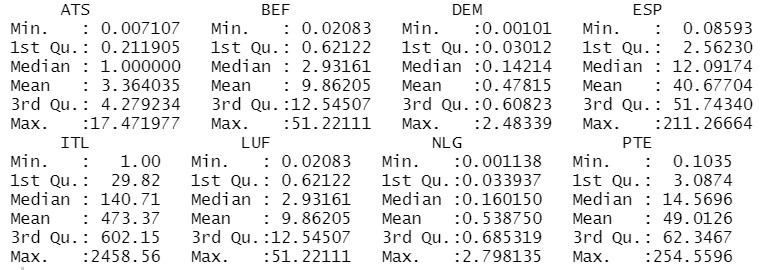
\includegraphics[scale=.8]{S1}
\label{fig:S1}
\end{figure}
\begin{figure}
\centering
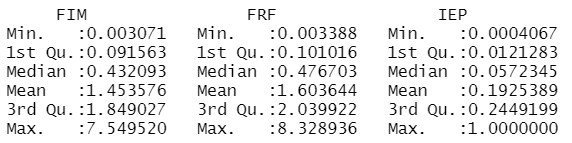
\includegraphics[scale=.8]{S2}
\caption{Summary}
\label{fig:S2}
\end{figure}
\newpage
\subsection{Graficas de densidad (Figura \ref{fig:G2})}
\begin{figure}
\centering
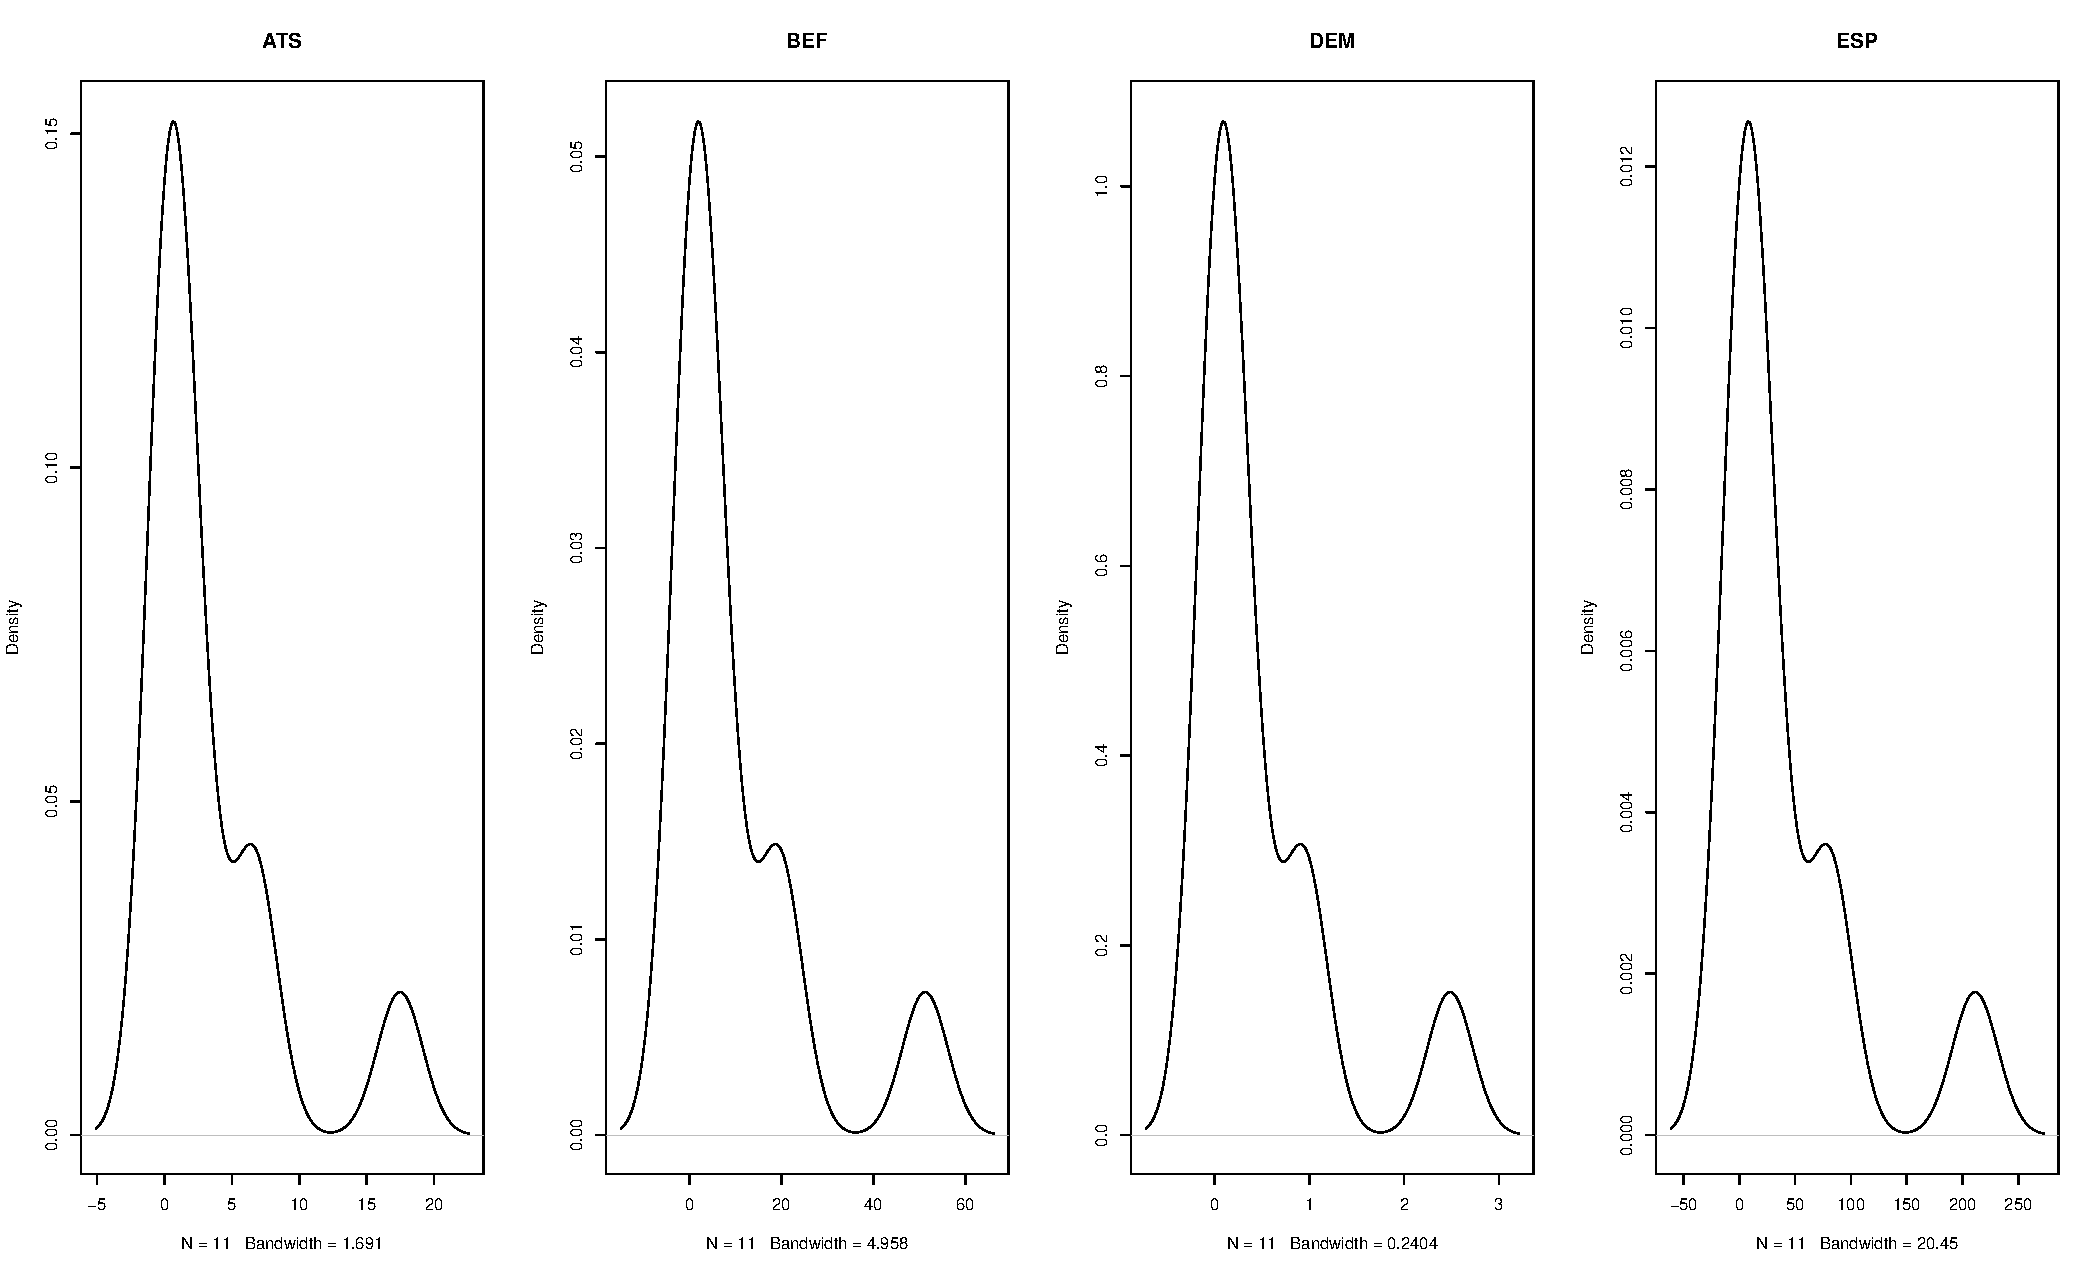
\includegraphics[scale=.5]{G2}
\caption{Densidad de 4 de las monedas respecto al euro}
\label{fig:G2}
\end{figure}
\newpage

\section{Conclusi\'{o}n}\label{sec:Con}
Gracias a esta practica conoci varias de las bases de datos que contiene R, asi como tambien aprendi un poco mas sobre la forma en la que debo de graficar y tambien sobre otras funciones de R como Summary. Esta base de datos la elegi debido a que considero que es bastante practica para cuando se realicen trabajos que involucren estas monedas. El codigo completo de R que utilice se encuentra en mi repositorio de Github \cite{repositorio}
\bibliography{BIBLIO}
\bibliographystyle{plainnat}

\end{document}